%Input preamble
%Style
\documentclass[12pt]{article}
\usepackage[top=1in, bottom=1in, left=1in, right=1in]{geometry}
\parindent 22pt
\usepackage{fancyhdr}

%Packages
\usepackage{adjustbox}
\usepackage{amsmath}
\usepackage{amsfonts}
\usepackage{amssymb}
\usepackage[english]{babel}
\usepackage{bm}
\usepackage[table]{xcolor}
\usepackage{tabu}
\usepackage{color,soul}
\usepackage[utf8x]{inputenc}
\usepackage{makecell}
\usepackage{longtable}
\usepackage{multirow}
\usepackage[normalem]{ulem}
\usepackage{etoolbox}
\usepackage{graphicx}
\usepackage{tabularx}
\usepackage{ragged2e}
\usepackage{booktabs}
\usepackage{caption}
\usepackage{fixltx2e}
\usepackage[para, flushleft]{threeparttablex}
\usepackage[capposition=top]{floatrow}
\usepackage{subcaption}
\usepackage{pdfpages}
\usepackage{pdflscape}
\usepackage[sort&compress]{natbib}
\usepackage{bibunits}
\usepackage[colorlinks=true,linkcolor=darkgray,citecolor=darkgray,urlcolor=darkgray,anchorcolor=darkgray]{hyperref}
\usepackage{marvosym}
\usepackage{makeidx}
\usepackage{setspace}
\usepackage{enumerate}
\usepackage{rotating}
\usepackage{epstopdf}
\usepackage[titletoc]{appendix}
\usepackage{framed}
\usepackage{comment}
\usepackage{xr}
\usepackage{titlesec}
\usepackage{footnote}
\usepackage{longtable}
\newlength{\tablewidth}
\setlength{\tablewidth}{9.3in}
\usepackage[bottom]{footmisc}
\usepackage{stackengine}
\newcommand\barbelow[1]{\stackunder[1.2pt]{$#1$}{\rule{1ex}{.085ex}}}
\usepackage{titletoc}
\usepackage{accents}
\usepackage{arydshln }
\usepackage{titletoc}
\titlespacing{\section}{.2pt}{1ex}{1ex}
\setcounter{section}{0}
\renewcommand{\thesection}{\arabic{section}}


\makeatletter
\pretocmd\start@align
{%
  \let\everycr\CT@everycr
  \CT@start
}{}{}
\apptocmd{\endalign}{\CT@end}{}{}
\makeatother
%Watermark
\usepackage[printwatermark]{xwatermark}
\usepackage{lipsum}
\definecolor{lightgray}{RGB}{220,220,220}
\definecolor{dimgray}{RGB}{105,105,105}

%\newwatermark[allpages,color=lightgray,angle=45,scale=3,xpos=0,ypos=0]{Preliminary Draft}

%Further subsection level
\usepackage{titlesec}
\titleformat{\paragraph}
{\normalfont\normalsize\bfseries}{\theparagraph}{1em}{}
\titlespacing*{\paragraph}
{0pt}{3.25ex plus 1ex minus .2ex}{1.5ex plus .2ex}

\titleformat{\subparagraph}
{\normalfont\normalsize\bfseries}{\thesubparagraph}{1em}{}
\titlespacing*{\subparagraph}
{0pt}{3.25ex plus 1ex minus .2ex}{1.5ex plus .2ex}

%Functions
\DeclareMathOperator{\cov}{Cov}
\DeclareMathOperator{\sign}{sgn}
\DeclareMathOperator{\var}{Var}
\DeclareMathOperator{\plim}{plim}
\DeclareMathOperator*{\argmin}{arg\,min}
\DeclareMathOperator*{\argmax}{arg\,max}

%Math Environments
\usepackage{amsthm}
\newtheoremstyle{mytheoremstyle} % name
    {\topsep}                    % Space above
    {\topsep}                    % Space below
    {\color{black}}                   % Body font
    {}                           % Indent amount
    {\itshape \color{dimgray}}                   % Theorem head font
    {.}                          % Punctuation after theorem head
    {.5em}                       % Space after theorem head
    {}  % Theorem head spec (can be left empty, meaning ?normal?)

\theoremstyle{mytheoremstyle}
\newtheorem{assumption}{Assumption}
\renewcommand\theassumption{\arabic{assumption}}

\theoremstyle{mytheoremstyle}
\newtheorem{assumptiona}{Assumption}
\renewcommand\theassumptiona{\arabic{assumptiona}a}

\newtheorem{assumptionb}{Assumption}
\renewcommand\theassumptionb{\arabic{assumptionb}b}

\newtheorem{assumptionc}{Assumption}
\renewcommand\theassumptionc{\arabic{assumptionc}c}

\theoremstyle{mytheoremstyle}
\newtheorem{lemma}{Lemma}

\theoremstyle{mytheoremstyle}
\newtheorem{proposition}{Proposition}

\theoremstyle{mytheoremstyle}
\newtheorem{corollary}{Corollary}

%Commands
\newcommand\independent{\protect\mathpalette{\protect\independenT}{\perp}}
\def\independenT#1#2{\mathrel{\rlap{$#1#2$}\mkern2mu{#1#2}}}
\newcommand{\overbar}[1]{\mkern 1.5mu\overline{\mkern-1.5mu#1\mkern-1.5mu}\mkern 1.5mu}
\newcommand{\equald}{\ensuremath{\overset{d}{=}}}
\captionsetup[table]{skip=10pt}
%\makeindex

%Table, Figure, and Section Styles
\captionsetup[figure]{labelfont={bf},name={Figure},labelsep=period}
\renewcommand{\thefigure}{\arabic{figure}}
\captionsetup[table]{labelfont={bf},name={Table},labelsep=period}
\renewcommand{\thetable}{\arabic{table}}
\titleformat{\section}{\centering \normalsize \bf}{\thesection.}{0em}{}%\titlespacing*{\subsection}{0pt}{0\baselineskip}{0\baselineskip}
\renewcommand{\thesection}{\arabic{section}}

\titleformat{\subsection}{\flushleft \normalsize \bf}{\thesubsection}{0em}{}
\renewcommand{\thesubsection}{\arabic{section}.\arabic{subsection}}

%No indent
\setlength\parindent{24pt}
\setlength{\parskip}{5pt}

%Logo
%\AddToShipoutPictureBG{%
%  \AtPageUpperLeft{\raisebox{-\height}{\includegraphics[width=1.5cm]{uchicago.png}}}
%}

\newcolumntype{L}[1]{>{\raggedright\let\newline\\\arraybackslash\hspace{0pt}}m{#1}}
\newcolumntype{C}[1]{>{\centering\let\newline\\\arraybackslash\hspace{0pt}}m{#1}}
\newcolumntype{R}[1]{>{\raggedleft\let\newline\\\arraybackslash\hspace{0pt}}m{#1}} 

\newcommand{\mr}{\multirow}
\newcommand{\mc}{\multicolumn}

%\newcommand{\comment}[1]{}

\begin{document}


\title{\Large \textbf{Does Entrepreneurship Mitigate or Exacerbate Social Mobility? }}
\author{Yi Ling}

\date{\today}

\maketitle

\thispagestyle{empty} 
\doublespacing
\thispagestyle{empty} 

\section{Introduction}

Entrepreneurship is a key source of innovation, as new firms generate more patents and introduce novel products and services \citep{autio2014entrepreneurial}. Entrepreneurship also creates substantial employment growth, which explains the strong policy interest in fostering entrepreneurial activity \citep{parker2006economics}. However, in recent decades, we have witnessed a decline in entrepreneurial activity \citep{jiang2023skill}. Prior research has categorized entrepreneurs in various ways: for instance, \citet{jiang2023skill} distinguishes entrepreneurs by skill level, while \citet{sanchez2023decline} separates them into corporate and unincorporated self-employment. However, few studies discuss the returns between nascent entrepreneurs and those who come from self-employed families. Compared with nascent entrepreneurs, individuals whose parents are self-employed tend to possess greater intangible capital and face fewer financial constraints \citep{quadrini1999importance}. Therefore, examining trends in the composition of the entrepreneurial population and the returns they earn may shed light on the broader decline in entrepreneurship.

From another perspective, entrepreneurs typically exhibit high wealth concentration \citep{cagetti2006entrepreneurship}, contributing to rising wealth inequality over time. Despite their high saving rates, entrepreneurial returns are often lower than public equity returns—a phenomenon known as the “private equity premium puzzle,” which highlights the relatively low returns earned by entrepreneurs in comparison with public equity investors \citep{moskowitz2002returns, bhandari2020survey}. Although many studies explore why individuals choose to become entrepreneurs despite earning lower returns \citep{parker2006economics, vereshchagina2009risk}, few examine heterogeneity in returns across different types of entrepreneurs, beyond the conventional distinction between corporate and unincorporated self-employment.

Therefore, having the right policy to support entrepreneurs who contribute more to the business dynamics is essential. This proposal aims to compare the investment returns of workers and two types of entrepreneurs:  first-generation entrepreneurs and entrepreneurs whose family is also self-employed, and examine whether the first type faces lower intergenerational mobility than the second type, in other words, can people from a non-entrepreneur family background climb up the social ladder through choosing to start a business?               


\section{Literature Review}
The first relates to the macroeconomic and public literature on determinants of entrepreneurship and entrepreneurial returns. The classic puzzle in macroeconomics is the "Private Equity Premium Puzzle" \citep{moskowitz2002returns, bhandari2020survey}. In other words, people will have higher returns if they choose to be a worker. Since they have lower returns, the reasons why people choose to be entrepreneurs are widely discussed \citep{parker2006economics, vereshchagina2009risk}. \citet{parker2006economics} summarizes these reasons and adds other explanations: entrepreneurs' future earnings are unaffected by their current business; entrepreneurs could tolerate the high risk in their businesses; entrepreneurship provides additional private benefits. Additionally, \citet{vereshchagina2009risk} suggested that non-concavity areas created in the interaction with an occupational choice between being an entrepreneur and an employee could explain the high risk in investment. This research also aims to calculate the returns of two types of entrepreneurial investment. Since the returns of two types of entrepreneurs might be different, this might be the reason why entrepreneurial returns are lower than workers. If first-generation entrepreneurs earn lower returns while those with parental self-employment backgrounds earn higher returns, then the apparent puzzle can be explained by the higher failure rate among first-generation entrepreneurs. 

The second relates to the entrepreneurship's impact on wealth concentration and inequality. \citet{quadrini1999importance} points out that entrepreneurship has implications for high wealth concentration: entrepreneurs have higher asset holdings even though their income is not larger than non-entrepreneurs. Moreover, entrepreneurs have greater upward mobility, which means they have a greater probability of moving to higher wealth classes, and this is not only due to their higher incomes. \citet{cagetti2006entrepreneurship} also emphasizes that the reason why entrepreneurs have higher wealth is because they save more for borrowing constraints, and share the fortune with their children to keep the family firm working. This research aims to find whether the saving patterns of two types of entrepreneurs are different, which leads to the high saving rate of entrepreneurs.

The third relates to the literature on social mobility. Intergenerational mobility has long been a central topic of interest for economists worldwide, as greater inequality in a society tends to make family background a stronger determinant of offspring’s outcomes \citep{corakIncomeInequalityEquality2013a}. There are many discussions on how parental self-employment impacts children's occupation decisions \citep{dunn2000financial, laferrere2001self, djankov2006china, barnir2011parental, lindquist2015entrepreneurial}. This research is most closely related to \citet{barnir2011parental, lindquist2015entrepreneurial}. \citet{barnir2011parental} compare first-generation self-employers and self-employers who have entrepreneurial parents, they found that through vicarious learning, people who have entrepreneurial parents can observe and learn from their family, which makes it easier to become an entrepreneur, but they face the same financial constraints when their firm enters the market.  \citet{lindquist2015entrepreneurial} also compares the difference between the entrepreneurs whose parents were self-employed and those whose parents were not, they found that parental entrepreneurship increases the probability of children’s entrepreneurship by about 60\% due to role modeling.  Other papers consider the occupation decision within the entrepreneur family. \citet{dunn2000financial, laferrere2001self, djankov2006china} found offspring of the self-employed display a greater propensity to become entrepreneurs. Previous literature also explores the intergenerational mobility in many other aspects \citep{peters1992patterns, checchi1999more}. For instance, \citet{chetty2018impacts} analyzes the neighborhood's impact on intergenerational mobility, finding out the outcome of the children is better when they spend their childhood in better opportunity areas.


\section{Data Description}
There are many data sources that provide information on income, profits, and investments for entrepreneurs and their family backgrounds. One prominent dataset is the Panel Study of Income Dynamics (PSID), a longitudinal household survey that began in 1968 and covers a nationally representative sample of over 18,000 individuals from 5,000 families in the United States. \citet{quadrini1999importance,fairlie1999absence} both use the  (PSID) to study the financial and human capital transition across generations. Specifically, \citet{fairlie1999absence} studies the black transition rate into self-employment using PSID, which is helpful when I construct the panel data.

The second dataset is the Current Population Survey (CPS), which is an important source of labor force data in the United States. To study the entrepreneurship trend, \citet{jiang2023skill, sanchez2023decline, bento2023barriers} both used CPS and found the decline trend in the entrepreneur population. Before calculating the income, investment of two types of entrepreneurs, I also calculated the population trend to ensure my definition of entrepreneurs is the same as previous literature. First, I only included the people who have an active employment status. Second, I define entrepreneurs as "self-employed" from the data. For family background, I only consider parents' employment status first, then I merge parents' employment information with the original data. Figure \ref{nascent} shows the population trend of nascent entrepreneurs, which is consistent with the results from \citet{jiang2023skill, sanchez2023decline}.

\begin{figure}[htp!]
    \centering
    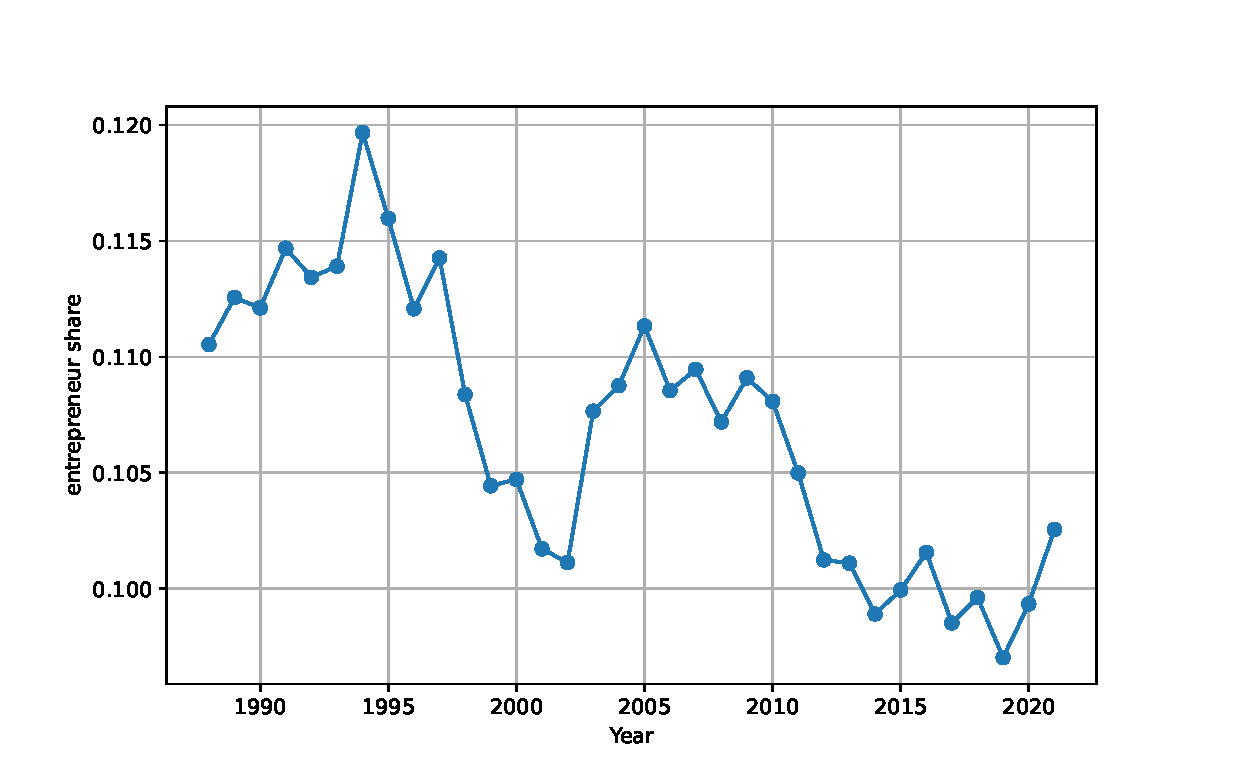
\includegraphics[width=5.5in]{nascententrepreneursharecps.eps}
    \caption{Population Trend of Nascent Entrepreneurs}
    \label{nascent}
\end{figure}

Another dataset is also helpful to identify the entrepreneur trend over time, but it cannot provide detailed information about the entrepreneurs' families. For instance, Survey of Consumer Finance (SCF) is also widely used to observe the entreprenuers population and investment \citep{moskowitz2002returns, cagetti2006entrepreneurship}, however, the question in the inverview is " How did you (or your family living here) first acquire this business; was it bought or invested in, started by you, inherited, given to you, or some other way?", therefore, we cannot identify whether the business is started by that person or his family. From my previous research, I replicated \citet{moskowitz2002returns, kartashova2014private}, which calculates the entrepreneurial returns and public returns, and I separated the entrepreneurs into corporate and unincorporated and extended the period. Table \ref{1} and Table \ref{2} show that, the overall returns of entrepreneurial investment are similar to the public returns, which is different from the conclusion from \citet{kartashova2014private}.

\begin{figure}
\centering
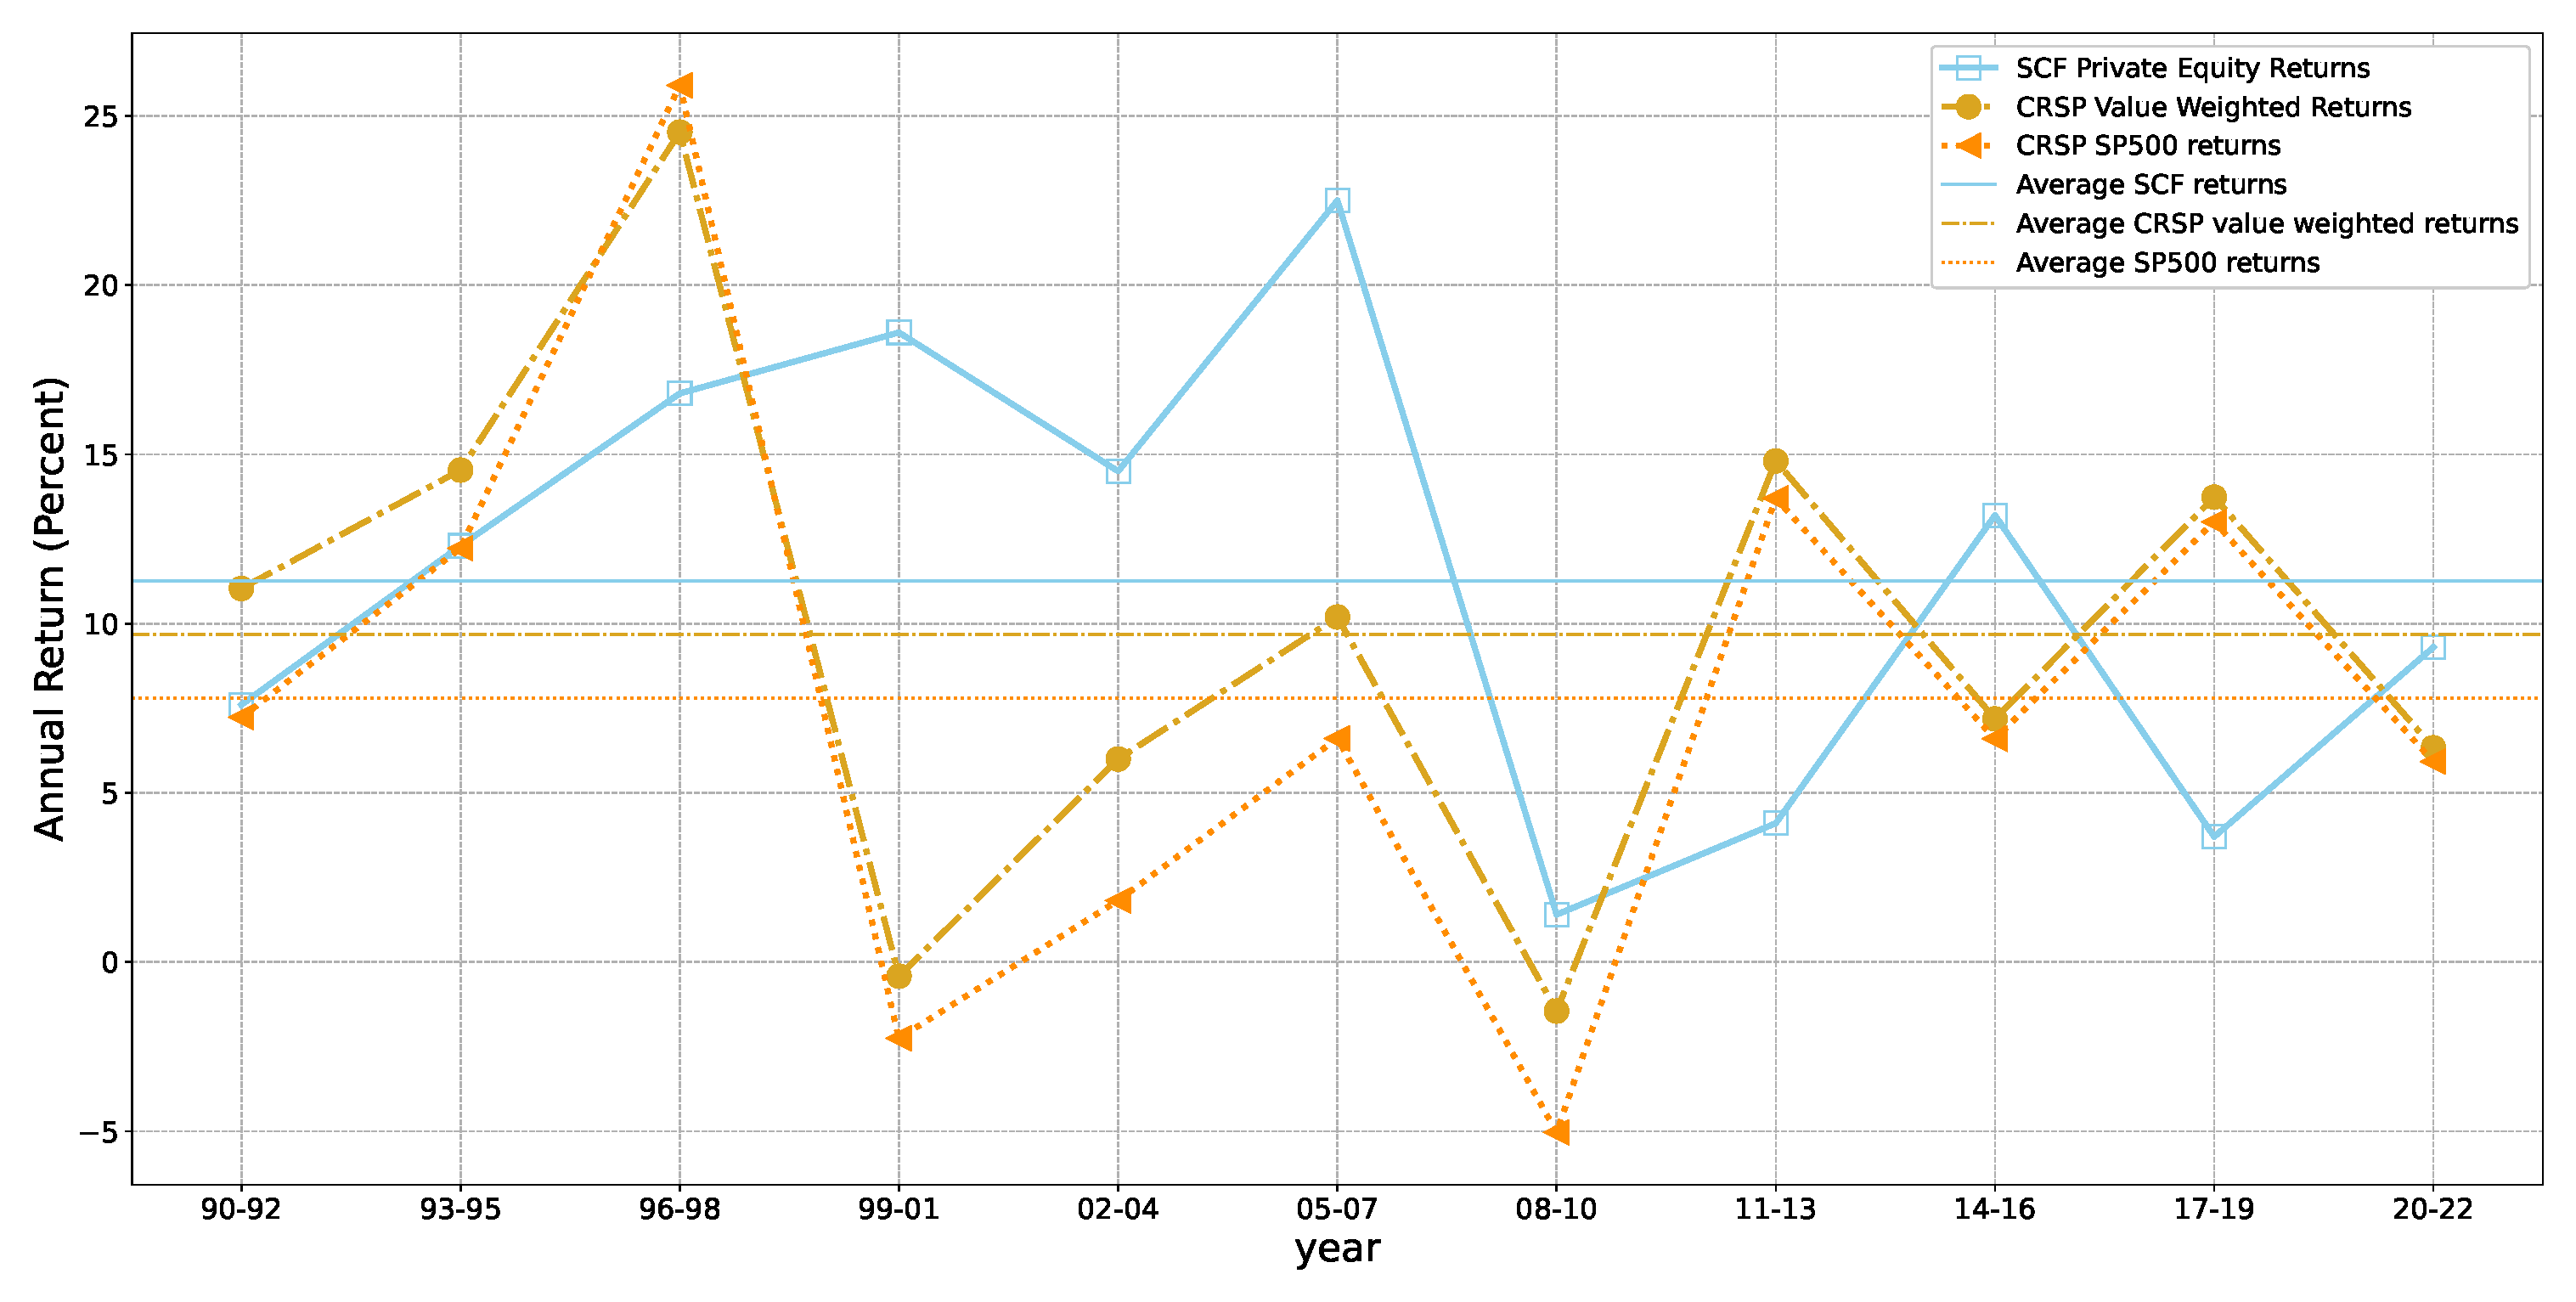
\includegraphics[width=5.5in]{scfandcrspreturns2.eps}
\caption{Comparison of Private and Public Equity Returns(1990$-$2022)}
\floatfoot{Notes: The figure depicts the trends and presents the average returns from the period of 90-92 to 20-22. Triennial returns in SCF are reported to calculate private equity returns from 90-92 period to 20-22 period. Annual data of value-weighted returns and S\&P 500 returns are transferred into triennial returns from the same period using CRSP.}
\label{1}
\end{figure}

\begin{figure}[htp!]
  \centering
  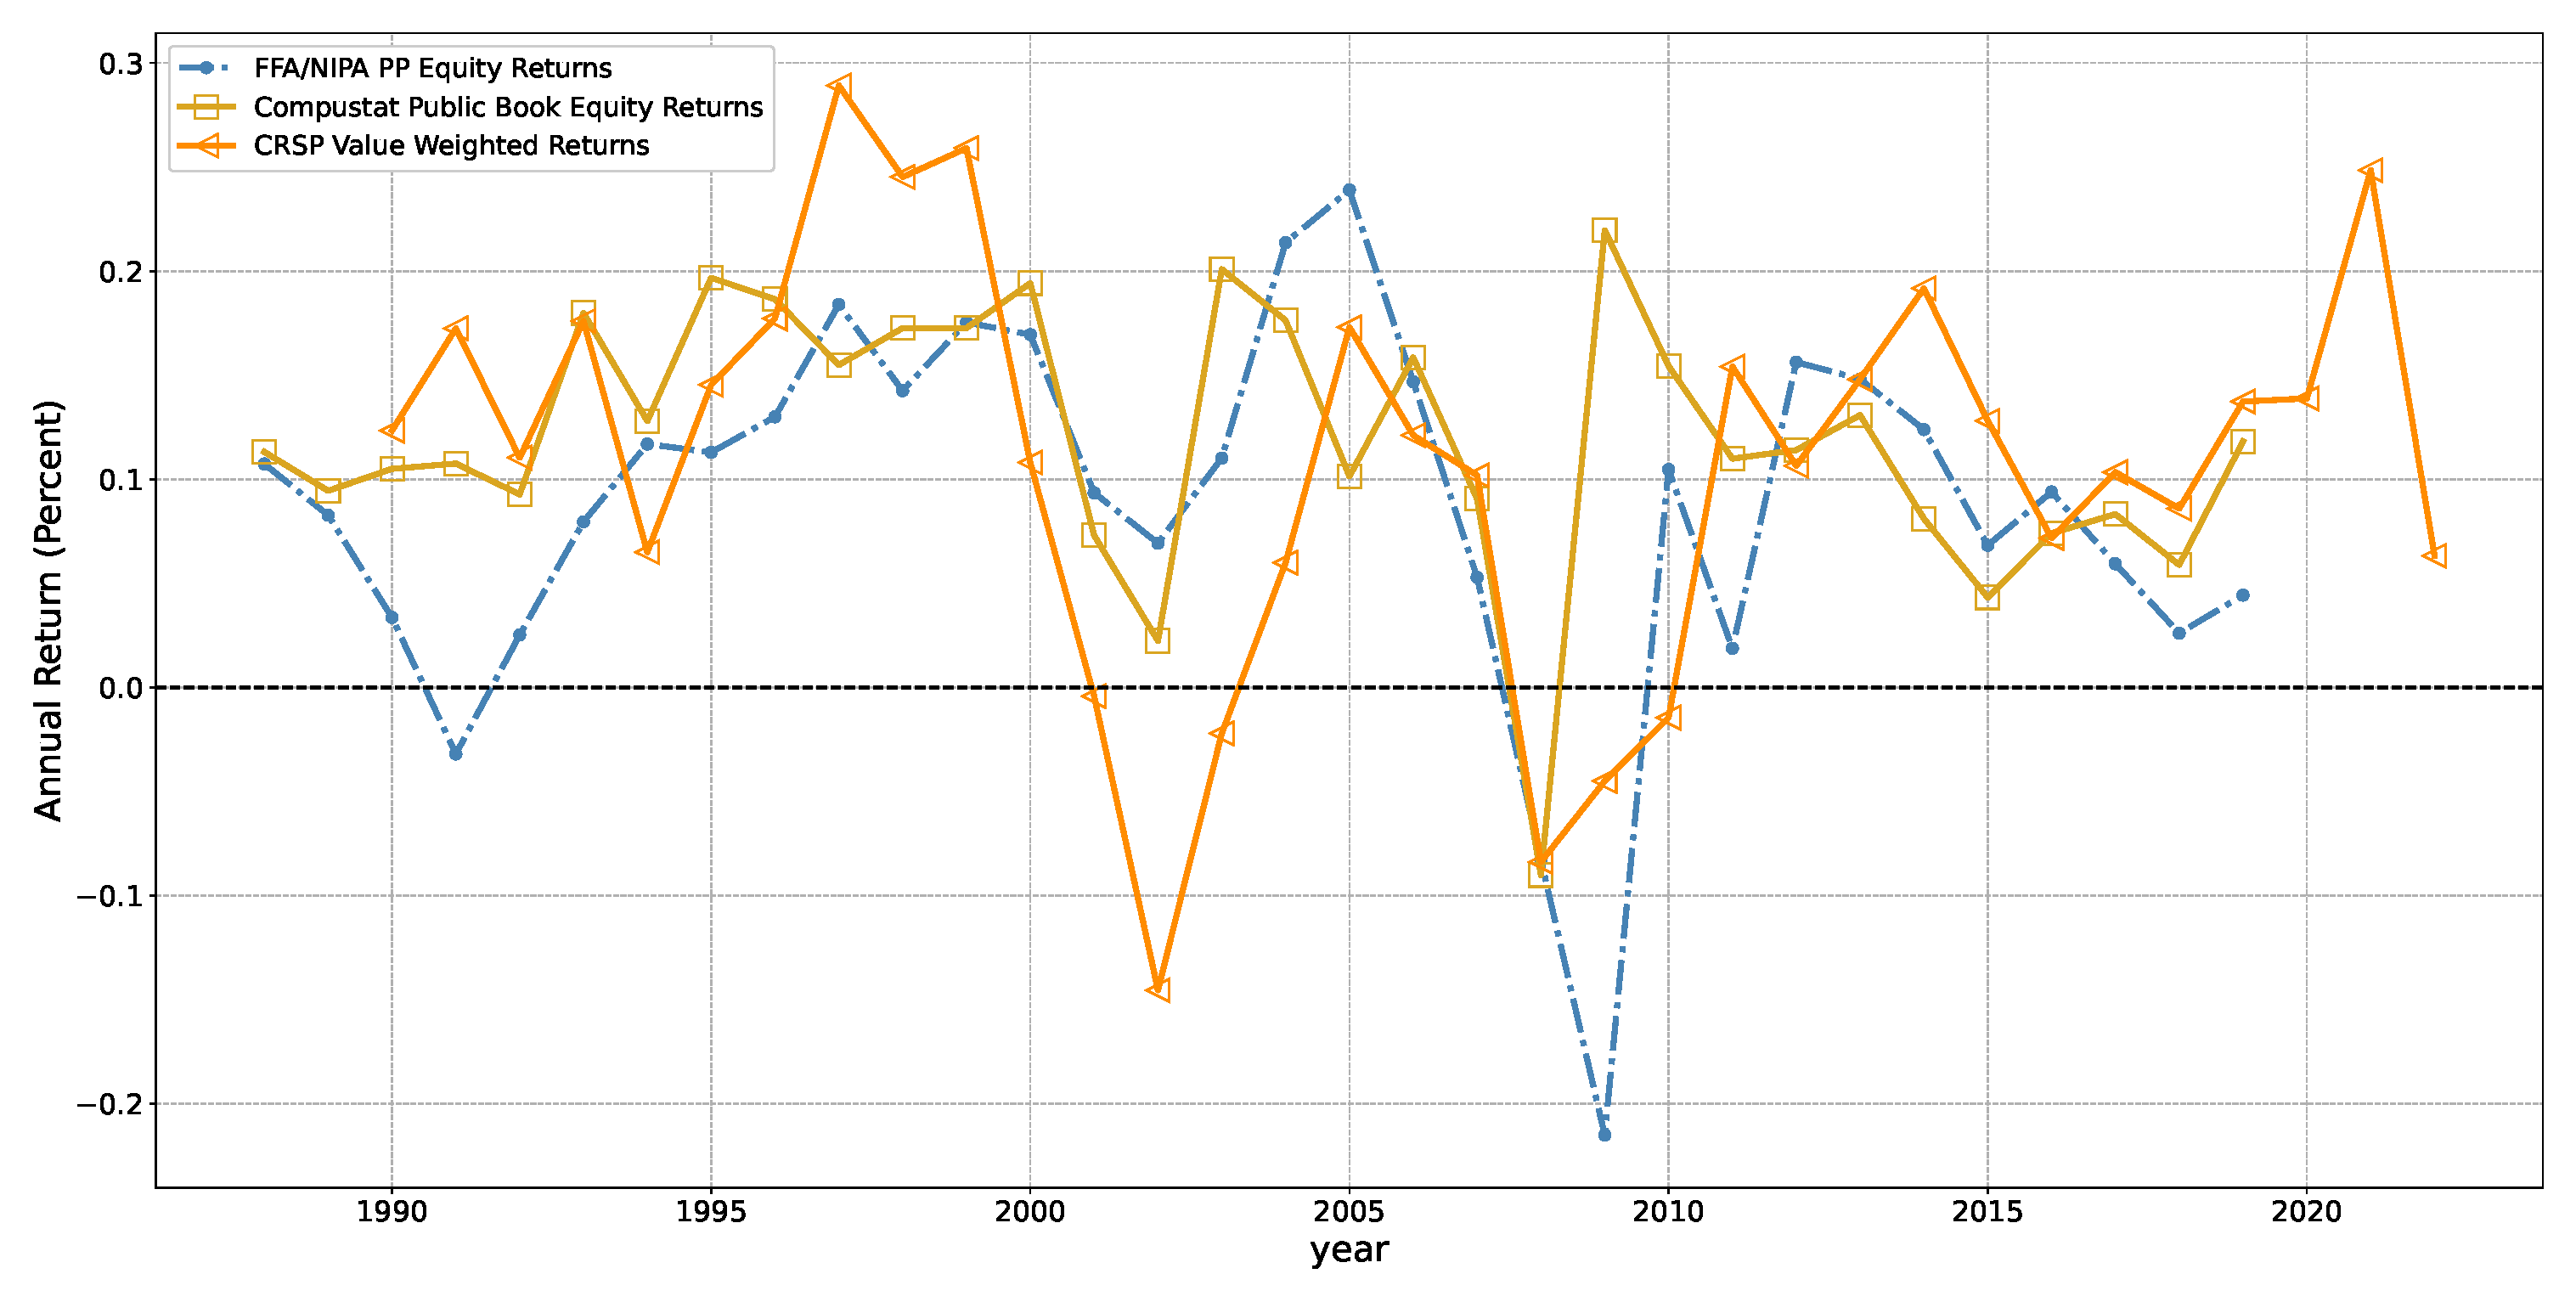
\includegraphics[width=5.5in]{private-and-public-returns2.eps}
  \caption{
    Longer Period: Comparison of Private and Public Equity Returns (1988--2019).
  }
 \floatfoot*{Notes: Trends of annual private market returns using FFA and NIPA, compared to public market returns are discussed. FFA and NIPA data are deployed to calculate proprietorship and partnership(P\&P) equity returns, from 1997 to 2019. For public equity returns, market values in CRSP data from 1990 to 2022 are employed to calculate value-weighted returns, and book returns of public equity are recorded from 1988 to 2019 using Compustat data.}
 \label{2}
\end{figure}


\section{Empirical Design}
The casualty strategy is designed to compare the returns of the worker and the two types of entrepreneurs. I adopt the same logit to calculate the returns from \citet{moskowitz2002returns}. With $\gamma$ as the retain earning rate,the capital gain is calculated in this way:

\begin{equation}
    Capital\ Gain _{i.t}=Profits _{i,t} (1-\gamma )-Wage _{i,t}
    \label{capital_gain}
\end{equation}

PSID also provides much information about the household head's wealth, which includes assets, stocks, and other real estate. Denote that we have $K$ types of assets, the equity of the entrepreneur $i$ in time $t$ is:

\begin{equation}
    Equity _{i,t}= \sum_{k=1}^{k=K} Assets _{ikt} 
    \label{market_value}
\end{equation}

Since PSID records the information every two years, the returns for the entrepreneur can be calculated:

\begin{equation}
R_{i,t+2} = \frac{\text{Equity}_{i,t+2} +  \text{Capital Gain}_{i,t+2}}{\text{Equity}_{i,t+1}} \label{eq:returns}
\end{equation}

For workers, since they earn salaries and can also make investments in public stocks, the return is calculated by:

\begin{equation}
R_{i,t+2} = \frac{\text{Equity}_{i,t+2} +  \text{Salaries}_{i,t+2}}{\text{Equity}_{i,t+1}} \label{eq:returns}
\end{equation}

Then, for each household, we have the returns each year either from business or from salaried work. Second, since both CPS and PSID provide annual information about their class of work, we can identify the year the household started the business. Therefore, an event study can be designed to see the impact of starting a business on the returns to work, and set up 6-year windows, comparing the returns 3 years before they chose to be an entrepreneur, and 3 years after they chose to become an entrepreneur. Specifically, the strategy is set in this way:

\begin{equation}
Y_{it} = \sum_{k \neq -1, k \in \mathcal{K}} \beta_{k,1} *\mathbf{1}[t-E_i = k]*\mathbf{1}[Type=1]+ \\ \sum_{k \neq -1, k \in \mathcal{K}} \beta_{k,2} *\mathbf{1}[t-E_i = k]*\mathbf{1}[Type=2]+\theta_{i} + \lambda_{t} + \epsilon_{it}
\end{equation}

In this model, $Y_{it}$ represents household returns, and $rel\_year$ denotes the number of years since the transition to entrepreneurship. The terms $\theta_{i}$ and $\lambda_{t}$ control for individual fixed effects and time fixed effects, respectively. 


\section{Expected Results}
I am working on merging the data from PSID. I finished merging the household individual data with family data for 2015, which linked family heads to their parents, yielding 468 child-father pairs. Within this sample, 44 children (9.4\%) are identified as entrepreneurs. Moreover, the rate of entrepreneurs each year is calculated and shown in Figure 2:

\begin{figure}[htp!]
    \centering
    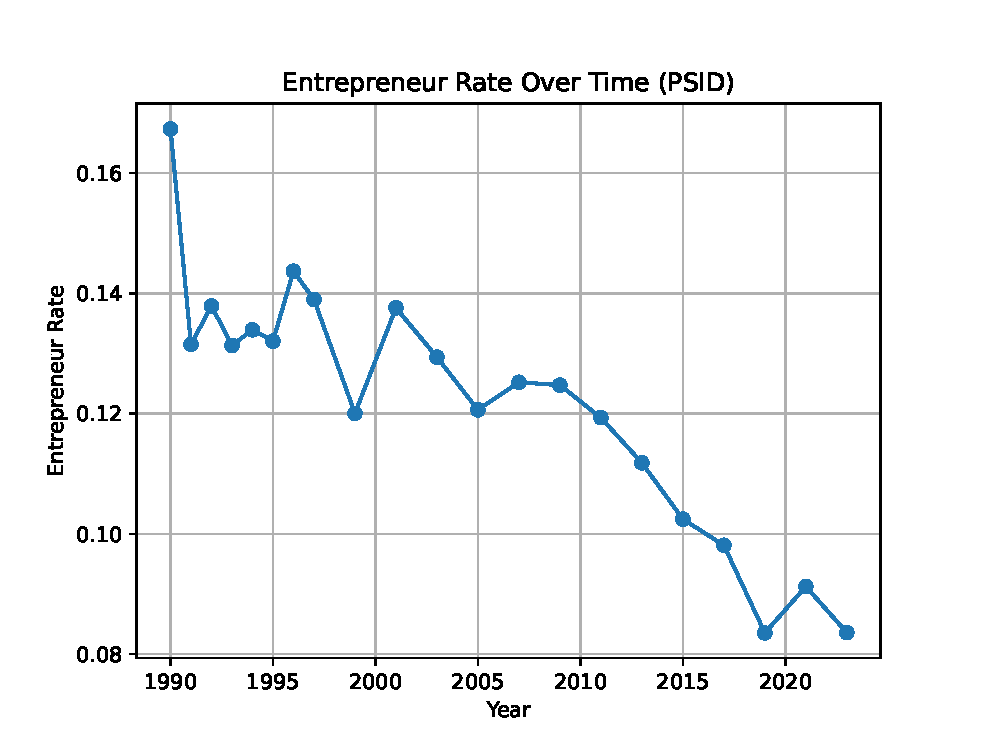
\includegraphics[width=5.5in]{entrepreneursharepsid.eps} 
    \caption{Population Trend of Entrepreneurs in PSID}
    \label{nascent_psid}
\end{figure}

 The subsequent steps involve merging data from other years and determining the parents' pre-transition employment status to prepare for the empirical strategy. Since PSID only provides the family head's occupation status, I need to connect the family head with his parents, who are also family heads. I successfully connect individual information with family information, as well as the individual's parents' information. The next step is finding parents' own family occupations and matching them together.

 \section{Conclusion}
After processing the data, this proposal can calculate two types of entrepreneurial returns and compare them with the returns of workers. First, the results can provide an explanation for the private equity premium puzzle. Second, the results can compare the returns with two types of entrepreneurs, which can show the generational transfer in entrepreneurship, which implies that future policy in supporting new start-ups should focus more on nascent entrepreneurs.

\bibliographystyle{apalike} 
\bibliography{references}

\end{document}

